% !TeX program = xelatex
%% ViCivil-TKG - paper NCKH (IMRaD). Biên dịch: tectonic (XeTeX).
%% Font: Liberation Serif (đủ dấu tiếng Việt). Cover merge riêng, không titlepage.
\documentclass[11pt,a4paper]{article}
\usepackage{fontspec}
\setmainfont{Liberation Serif}
\setsansfont{Liberation Sans}
\setmonofont{Liberation Mono}[Scale=0.92]
\usepackage{polyglossia}
\setdefaultlanguage{vietnamese}
\setotherlanguage{english}
\usepackage[a4paper,left=2.5cm,right=2.5cm,top=2.4cm,bottom=2.4cm]{geometry}
\usepackage{amsmath,amssymb}
\usepackage{booktabs}
\usepackage{graphicx}
\usepackage{tikz}
\usetikzlibrary{arrows.meta,positioning,shapes.multipart}
\usepackage{array}
\usepackage{multirow}
\usepackage{xcolor}
\usepackage[hidelinks]{hyperref}
\usepackage{caption}
\captionsetup{font=small,labelfont=bf}
\usepackage{titlesec}
\titleformat{\section}{\large\bfseries}{\thesection.}{0.6em}{}
\titleformat{\subsection}{\normalsize\bfseries}{\thesubsection.}{0.6em}{}
\setlength{\parskip}{2pt}
\setlength{\tabcolsep}{4.5pt}
\setlength{\emergencystretch}{2em}

% - Okabe-Ito palette (giống bản EN, an toàn màu mù) -
\definecolor{cblue}{RGB}{0,114,178}
\definecolor{cverm}{RGB}{213,94,0}
\definecolor{cgreen}{RGB}{0,158,115}
\definecolor{corange}{RGB}{230,159,0}
\definecolor{cpurple}{RGB}{204,121,167}
\definecolor{csky}{RGB}{86,180,233}
\definecolor{cgrayN}{RGB}{90,98,112}
\newcommand{\btxt}{\fontsize{6.4}{7.6}\selectfont}
\newcommand{\stagelbl}[1]{\color{#1!85!black}\fontsize{6.9}{8.0}\selectfont\bfseries}

\begin{document}

\begin{center}
{\LARGE\bfseries ViCivil-TKG: Bộ chuẩn đánh giá hệ thống hỏi-đáp\\[2pt] pháp luật dân sự Việt Nam với kiểm định thời hiệu\\[2pt] và chuỗi thẩm định đáp án vàng đa vòng\par}
\vspace{6pt}
{\normalsize Nhóm nghiên cứu ViCivil-TKG\par}
\vspace{2pt}
{\small Kho dữ liệu và mã nguồn: \url{https://huggingface.co/datasets/datbazuka2502/vicivil-tkg} - \url{https://github.com/ntd25022006q/vicivil-tkg}\par}
\end{center}

\vspace{4pt}

\noindent\textbf{Tóm tắt.} Chúng tôi giới thiệu \textbf{ViCivil-TKG}, bộ chuẩn đánh giá (benchmark) cho bài toán hỏi-đáp pháp luật dân sự Việt Nam, được xây dựng quanh hai thách thức ít được xử lý trong các bộ dữ liệu pháp lý hiện có: (i) \emph{thời hiệu văn bản} - cùng một câu hỏi có đáp án khác nhau tại các mốc thời gian áp dụng khác nhau của đạo luật; và (ii) \emph{độ tin cậy của đáp án vàng} - phần lớn câu hỏi sinh tự động có đáp án vàng chưa được kiểm chứng độc lập. Bộ chuẩn gồm \textbf{1.092 câu hỏi} đã công bố (281 câu lõi trong đó 12 câu viết tay và 269 câu sinh có kiểm soát; 106 câu mở rộng vòng~1; 64 câu mở rộng vòng~2 thuộc giai đoạn văn bản 1996-2015; 265 câu mở rộng vòng~3 và 376 câu vòng~4 mở rộng quy mô) trích từ kho 20 văn bản pháp luật với 13.151 đoạn văn bản, kèm 1.029 câu bị cách ly công khai vì không qua thẩm định. Toàn bộ đáp án vàng trải qua chuỗi thẩm định bốn tầng: thẩm định hai tầng bằng hai mô hình giám sát, thẩm định lại hai vòng bằng LLM trọng số lớn hơn, và một lượt rà soát lần cuối (pass-3) bằng mô hình sâu hơn trên 99 câu nghi vấn cùng bài kiểm tra thỏa thuận độc lập trên 60 câu mẫu; sau chuỗi này \emph{không còn câu hỏi nào ở trạng thái ``không xác minh được''}. Trên bộ lõi, cơ chế lọc thời hiệu (TCR) cải thiện độ chính xác trích dẫn của mô hình sinh Qwen2.5-3B từ 0,488 lên 0,601 (McNemar $p=5{,}8\times10^{-5}$), so với 0,004 của thiết lập không có ngữ cảnh; với cohort mở rộng giai đoạn 1996-2015, TCR nâng Hit@5 truy hồi từ 0,703 lên 0,781 và rerank đưa Hit@1 lên 0,703; trên hai cohort mở rộng quy mô (vòng~3/4, 641 câu), TCR nâng Hit@1 truy hồi 0,511$\rightarrow$0,654 (vòng~4, $p=6{,}3\times10^{-22}$) và cite\_acc 0,527$\rightarrow$0,657 (vòng~4, $p=3{,}2\times10^{-10}$). Bộ dữ liệu, toàn bộ dấu vết thẩm định và kịch bản tái lập không cần GPU được công bố công khai.

\smallskip
\noindent\textbf{Từ khoá:} hỏi-đáp pháp lý; bộ dữ liệu tiếng Việt; truy hồi có thời hiệu; thẩm định đáp án vàng; RAG.

\smallskip
\noindent\textbf{Abstract.} We introduce \textbf{ViCivil-TKG}, a benchmark for Vietnamese civil-law question answering built around two under-addressed challenges: (i) \emph{temporal validity} - the same question has different answers under different applicability windows of a statute; and (ii) \emph{gold-label reliability} - most automatically generated questions carry unverified gold answers. The benchmark publishes \textbf{1,092 validated questions} (a 281-question core with 12 hand-written and 269 controlled-generated items; 106 round-1 extension items; 64 round-2 extension items from the 1996-2015 statute era; 265 round-3 and 376 round-4 scale-up items) over a corpus of 20 legal documents with 13{,}151 passages, together with \textbf{1,029 publicly quarantined questions} that failed adjudication. Every gold answer passes a four-stage adjudication chain: two-tier LLM auditing, two-round re-anchoring with a larger judge, a pass-3 sweep over 99 weak-gold suspects with guardrails, and an independent 60-question agreement audit; afterwards \emph{no question remains unverifiable}. On the core set, temporal-consistency retrieval (TCR) raises the citation accuracy of Qwen2.5-3B from 0.488 to 0.601 (McNemar $p=5.8\times10^{-5}$) against 0.004 without context; on the 1996-2015 extension cohort TCR lifts Hit@5 retrieval from 0.703 to 0.781 and reranking raises Hit@1 to 0.703; on the round-3/4 scale-up cohorts (641 questions) TCR raises Hit@1 from 0.511 to 0.654 (round 4, $p=6.3\times10^{-22}$) and cite\_acc from 0.527 to 0.657 (round 4, $p=3.2\times10^{-10}$). Data, full adjudication trails, and a GPU-free reproduction script are released.

\smallskip
\noindent\textbf{Keywords:} legal question answering; Vietnamese datasets; temporal retrieval; gold-label adjudication; RAG.

\section{Giới thiệu}

Hệ thống hỏi-đáp pháp luật đòi hỏi mức độ chính xác cao hơn nhiều so với các miền mở: một câu trả lời sai điều luật áp dụng có thể dẫn tới hậu quả pháp lý thực tế. Xây dựng bộ đánh giá cho miền này gặp hai rào cản chính. Thứ nhất, văn bản pháp luật Việt Nam có \emph{thời điểm hiệu lực} rõ ràng: Bộ luật Dân sự 2015 thay thế Bộ luật Dân sự 2005, nghị định hướng dẫn bị thay mới theo chu kỳ, do đó câu hỏi ``thời hiệu khởi kiện yêu cầu đòi tài sản là bao lâu?'' phải được trả lời bằng văn bản hợp lệ \emph{tại mốc thời gian của câu hỏi}, không phải bằng văn bản mới nhất. Thứ hai, các bộ dữ liệu QA sinh tự động bằng LLM phần lớn mặc định đáp án vàng (gold) là đúng, trong khi thực tế việc neo vàng (gold anchoring) - chỉ ra đúng đoạn văn bản là cơ sở pháp lý - là chính nguồn lỗi lớn nhất.

Bài báo này trình bày ViCivil-TKG, bộ chuẩn được thiết kế để đo cả hai khía cạnh trên. Đóng góp của chúng tôi gồm: (C1) bộ chuẩn 1.092 câu hỏi công bố trên kho 20 văn bản pháp luật dân sự Việt Nam (13.151 đoạn), mỗi câu gắn mốc thời gian \texttt{as\_of} và đáp án vàng neo tới định danh đoạn văn bản chính xác, cùng 1.029 câu cách ly công khai; (C2) \emph{chuỗi thẩm định vàng đa tầng} - một quy trình bốn tầng với nhiều mô hình giám sát độc lập, guardrail khi áp dụng, dấu vết provenance đầy đủ và cơ chế cách ly công khai các câu không đạt; (C3) giao thức đánh giá truy hồi có kiểm định thời hiệu (TCR) cùng phép thử thống kê cặp cho cả truy hồi lẫn sinh; (C4) phân tích lỗi theo tầng chất lượng vàng và kịch bản tái lập hoàn toàn không cần GPU.

Bài báo được tổ chức như sau: Mục~2 tóm tắt công trình liên quan; Mục~3 mô tả kho văn bản và quy trình sinh - thẩm định dữ liệu; Mục~4 trình bày thiết lập thực nghiệm; Mục~5 báo cáo kết quả; Mục~6 thảo luận hạn chế; Mục~7 kết luận.

\section{Công trình liên quan}

\textbf{Bộ chuẩn truy hồi và QA.} BEIR~\cite{thakur2021beir} chuẩn hoá đánh giá zero-shot cho truy hồi trên nhiều miền; LexGLUE~\cite{chalkidis2022lexglue} gom các tác vụ NLP pháp lý tiếng Anh. Các bộ này không có phân đoạn thời hiệu, không có văn bản tiếng Việt, và đáp án vàng được kiểm chứng bởi con người với chi phí cao - khác với hướng đi sinh có kiểm soát kèm thẩm định đa vòng của chúng tôi. SQuAD~2.0~\cite{rajpurkar2018squad} đưa câu hỏi ``không có đáp án'' vào đánh giá, gần với cơ chế từ chối trả lời (abstain) mà chúng tôi đo thông qua tỷ lệ trả lời ``Không đủ thông tin''.

\textbf{Truy hồi dày đặc và hợp nhất.} BM25~\cite{robertson2009bm25} vẫn là cơ sở truy hồi từ kho mạnh; DPR~\cite{karpukhin2020dpr} và các mô hình embedding dày đặc bổ sung tín hiệu ngữ nghĩa; Reciprocal Rank Fusion~\cite{cormack2009rrf} hợp nhất hai danh sách xếp hạng mà không cần huấn luyện lại. Chúng tôi dùng đúng tổ hợp BM25 + dense + RRF cho mọi thí nghiệm, và thêm lớp lọc thời hiệu (TCR) dựa trên đồ thị thời gian của văn bản. BGE-reranker~\cite{xiao2024cpack} được dùng làm bước xếp hạng lại; RAG~\cite{lewis2020rag} và dòng mô hình Qwen~\cite{yang2024qwen25} là nền cho điều kiện sinh có trích dẫn.

\section{Bộ dữ liệu ViCivil-TKG}

\subsection{Kho văn bản pháp luật}

Kho văn bản gồm 20 văn bản pháp luật dân sự Việt Nam giai đoạn 1995-2026 (Bộ luật Dân sự 1995/2005/2015, Bộ luật Tố tụng dân sự 2004 và VBHN, Luật Hôn nhân và gia đình 2000/2014, Luật Thi hành án dân sự 2008 và VBHN, Luật Nuôi con nuôi 2010, Luật Trách nhiệm bồi thường của Nhà nước, nghị định hướng dẫn, văn bản hợp nhất, cùng các văn bản 2026 mới ban hành), được phân đoạn thành \textbf{13.151 đoạn} theo cấu trúc điều - khoản - điểm. Mỗi đoạn mang các trường provenance bắt buộc: \texttt{source\_url}, \texttt{source\_type} (official / official-copy / semi-official / mirror), \texttt{fetched}, và cửa sổ hiệu lực \texttt{valid\_from}/\texttt{valid\_to} lấy từ đồ thị thời gian gồm 37 văn bản với 24 cạnh nối tiếp - sửa đổi, được vẽ đầy đủ trong Hình~\ref{fig:tkg}: mỗi đỉnh là một văn bản với cửa sổ hiệu lực của nó, mỗi cạnh là quan hệ thay thế - hợp nhất, và TCR chỉ giữ lại ứng viên mà cửa sổ hiệu lực chứa \texttt{as\_of} của câu hỏi. Hai đoạn trích từ tệp \texttt{.doc} chuyển đổi hỏng (nội dung nhiễu nhị phân, không được tham chiếu bởi bất kỳ câu hỏi nào) đã bị loại và ghi vào nhật ký loại bỏ.

\begin{figure}[t]
\centering
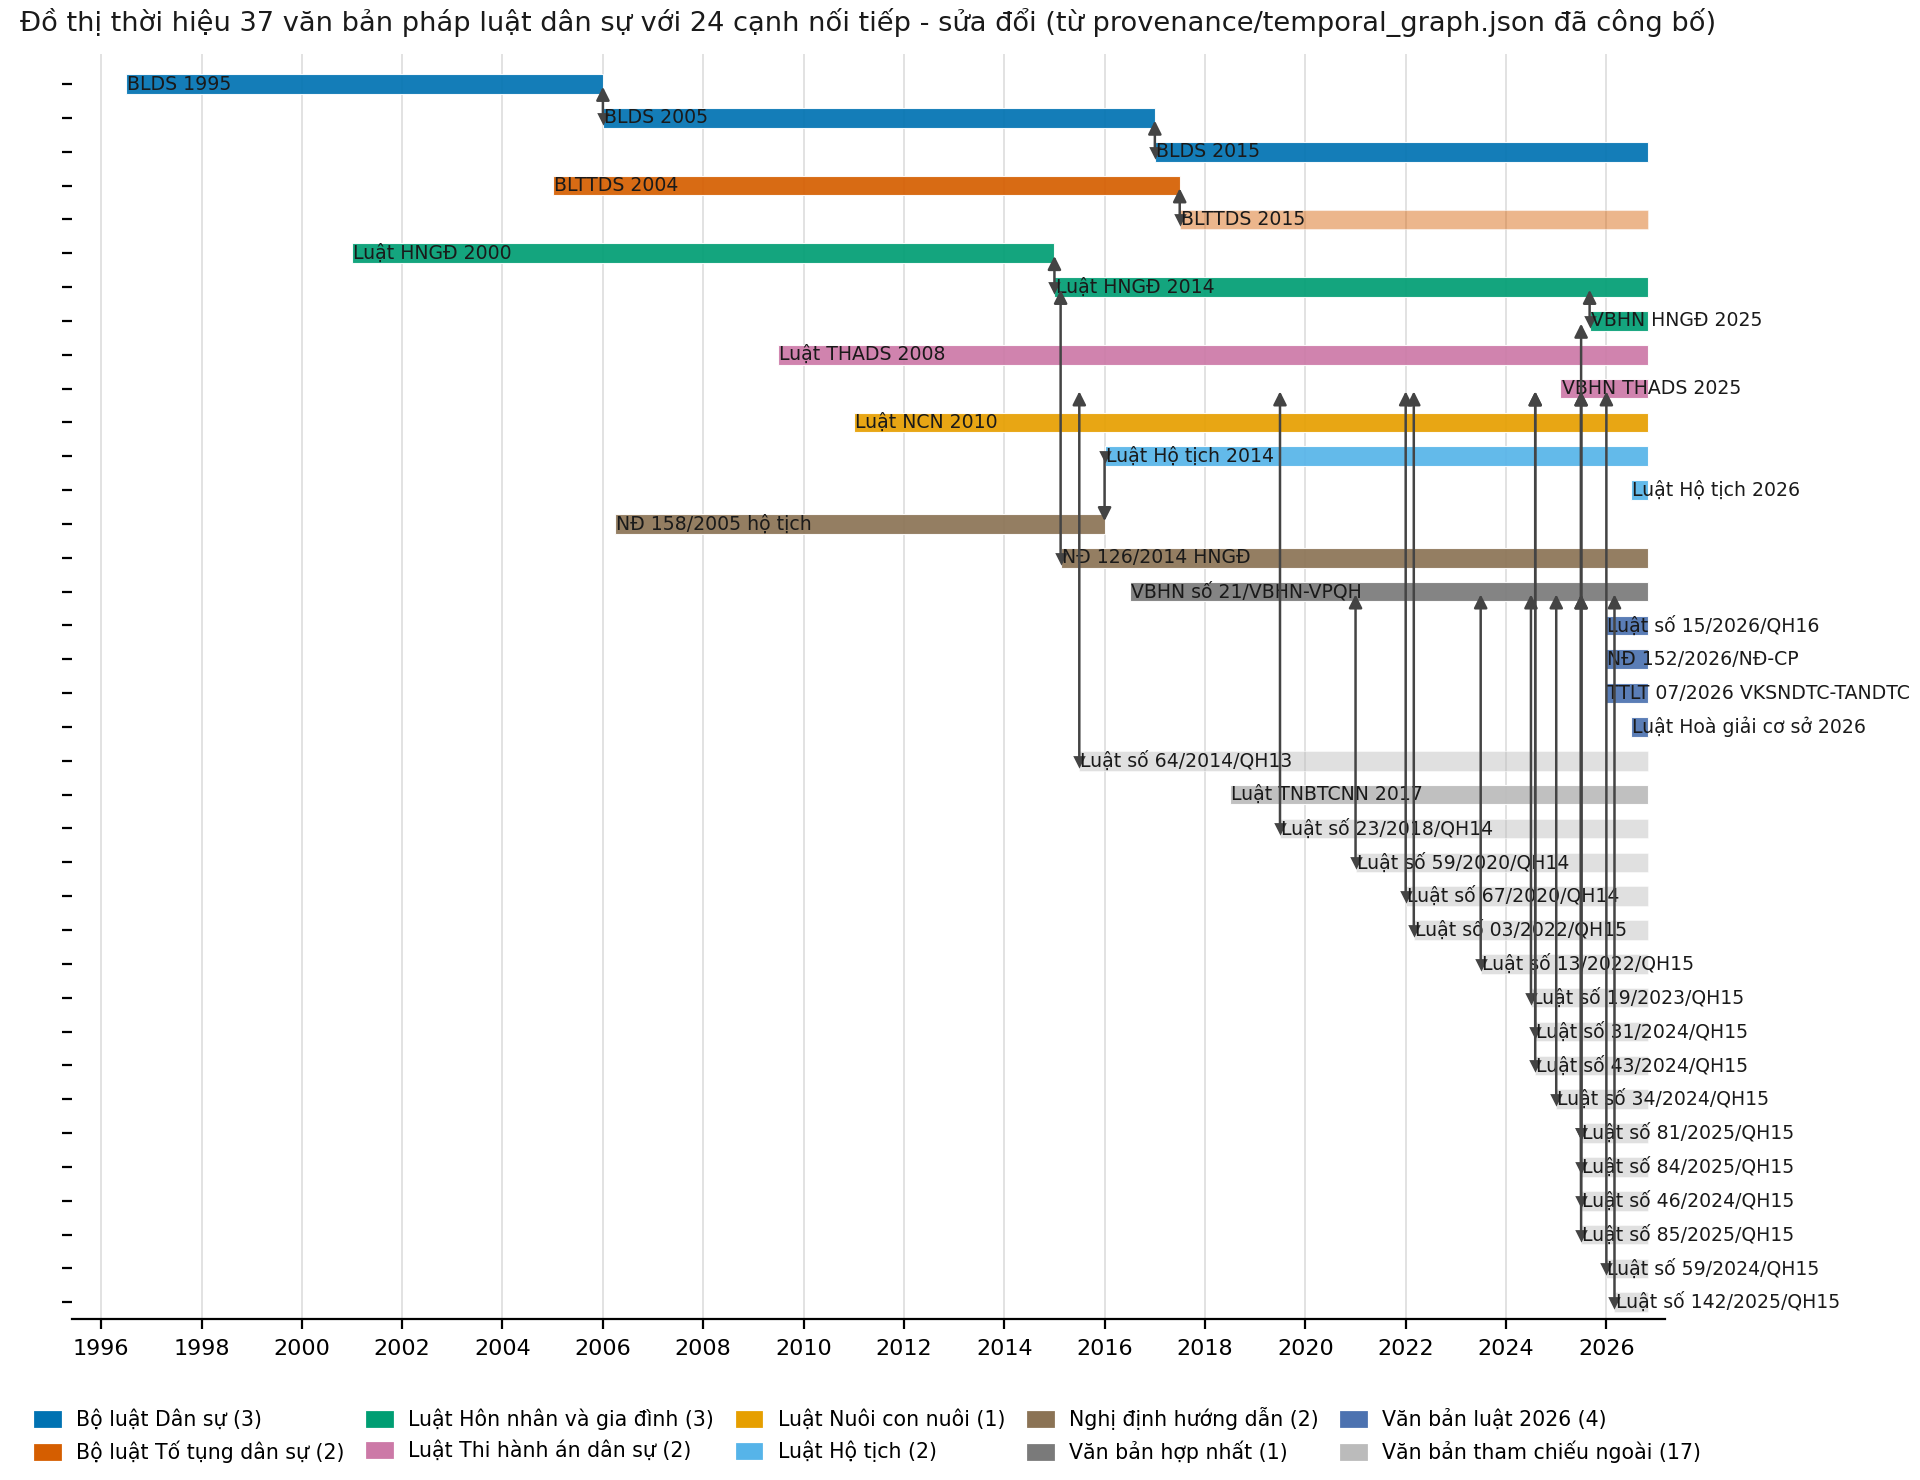
\includegraphics[width=0.97\linewidth]{figures/fig_temporal_graph.png}
\caption{Đồ thị thời hiệu của kho văn bản: 37 đỉnh (văn bản) với cửa sổ hiệu lực \texttt{valid\_from}/\texttt{valid\_to} và 24 cạnh nối tiếp - sửa đổi, vẽ trực tiếp từ \texttt{provenance/temporal\_graph.json} đã công bố. Ba thế hệ Bộ luật Dân sự 1995/2005/2015 nối tiếp nhau trọn vẹn; mũi tên chỉ thời điểm văn bản kế tiếp có hiệu lực; trục ngang là thời gian, thanh ngang là cửa sổ áp dụng.}
\label{fig:tkg}
\end{figure}

\subsection{Sinh câu hỏi có kiểm soát}

Câu hỏi được sinh bằng mô hình \texttt{qwen2.5:14b} chạy cục bộ, theo lô từ đoạn nguồn với ba ràng buộc: (i) mỗi câu gắn \texttt{as\_of} nằm trong cửa sổ hiệu lực của văn bản nguồn (chọn điểm giữa pha hữu dụng của văn bản); (ii) câu hỏi phải được trả lời được \emph{chỉ từ} đoạn nguồn và các điều liên hệ trực tiếp; (iii) dedup bên trong lô bằng vector câu hỏi (embedding 768 chiều, \texttt{embeddinggemma:300m}). Câu lõi gồm 269 câu sinh trên 14 văn bản có hiệu lực gần đây cộng 12 câu viết tay (CIV001-CIV012) dùng làm bài kiểm tra đặc biệt (trong đó một câu kiểm tra khả năng từ chối khi văn bản chưa hiệu lực). Hai đợt mở rộng bổ sung 106 câu công bố (vòng~1, từ 242 câu sinh) và 154 câu sinh từ ba văn bản giai đoạn 1996-2015 (Bộ luật Tố tụng dân sự 2004, Nghị định 158/2005 về hộ tịch, Nghị định 126/2014 hướng dẫn Luật HNGD) với quota theo văn bản là 103/30/27. Đợt mở rộng quy mô (vòng~3) lấy mẫu 620 đoạn theo quota từng văn bản (tối đa 150/văn bản), sinh 590 câu hợp lệ, loại 9 câu gần trùng lặp (Jaccard $\ge$ 0,60 với mọi câu trước đó) và công bố 265 câu sau cùng chuỗi thẩm định hai tầng và neo lại; 316 câu bị cách ly. Bài audit phát hành phát hiện 28 va chạm định danh câu hỏi do sinh song song (hai câu khác nhau dùng chung một ID khiến verdict lưu không tin cậy); mọi cặp bị ảnh hưởng được thẩm định lại từ đầu với ID duy nhất và nhật ký sửa được công bố.

\subsection{Chuỗi thẩm định đáp án vàng}

Đây là đóng góp trung tâm của bộ dữ liệu; Hình~\ref{fig:pipeline} tóm tắt toàn bộ chuỗi. Chuỗi gồm các tầng sau, toàn bộ dấu vết lưu trong \texttt{benchmark/}:

\begin{enumerate}
\item \textbf{Thẩm định hai tầng khi sinh.} Mỗi câu sinh được chấm ngay bởi mô hình 8B (\texttt{usable: yes/partial/no}); mọi câu không đạt ``yes'' được chấm lại bởi mô hình sâu hơn 14B kèm yêu cầu trích bằng chứng. Câu nào không qua cả hai tầng bị cách ly.
\item \textbf{Neo lại hai vòng.} Với các câu vàng nghi vấn, quy trình neo lại (regold) đề xuất đoạn thay thế rồi yêu cầu LLM giám sát xác nhận \emph{hai vòng độc lập}; chỉ đoạn được cả hai vòng chấp nhận mới được đổi. Trên bộ lõi, 38 câu được neo lại theo cách này (thỏa thuận giữa hai vòng 0,888).
\item \textbf{Pass-3: rà soát cuối trên 99 câu nghi vấn.} Toàn bộ nhóm vàng yếu nghi vấn (các câu chưa từng xác minh được, các câu đã regold, nhóm câu nhiều phần, nhóm viết tay) được một thẩm định viên sâu hơn (\texttt{qwen3:14b}) chấm lại theo giao thức ``gold hiện tại + 8 ứng viên truy hồi đã lưu'': kết luận \emph{gold-ok} (66 câu), \emph{reanchor} (3, cộng 1 đề xuất bị guardrail chặn vì không nằm trong danh sách ứng viên), hay \emph{flag} (29). Việc áp dụng đi kèm guardrail nghiêm ngặt: đoạn thay thế phải tồn tại trong kho, phải nằm trong danh sách ứng viên đã lưu, và phải hợp lệ theo cửa sổ thời hiệu tại \texttt{as\_of}.
\item \textbf{Kiểm tra thỏa thuận độc lập.} Trên mẫu ngẫu nhiên cố định 60 câu (seed 20261101), thẩm định viên độc lập chọn cơ sở pháp lý trong 8 ứng viên: 56/60 câu có kết quả phân tích được, trong đó 31/56 chọn đúng tập vàng (\textbf{0,554}) và 32/56 trùng khớp đoạn chính xác (\textbf{0,571}). Chúng tôi công bố con số này \emph{không lọc} như một thước đo độ khó gắn vàng của miền, đồng thời nhấn mạnh đây là kiểm tra giữa hai mô hình, không thay thế đánh giá giữa người (Mục~6).
\end{enumerate}

\begin{figure}[t]
\centering
\begin{tikzpicture}[
  font=\footnotesize, >={Stealth[length=2.4mm]},
  stage/.style={draw=#1!80!black, fill=#1!7, line width=0.7pt,
                rounded corners=1.8pt, align=center, inner sep=3.2pt,
                text width=2.34cm, minimum height=21mm},
  input/.style={stage=cgrayN},
  term/.style={draw=cgreen!75!black, fill=cgreen!10, line width=1.0pt,
               rounded corners=1.8pt, align=center, inner sep=3.2pt,
               text width=2.34cm, minimum height=21mm},
  exit/.style={draw=#1!75!black, fill=white, line width=0.7pt,
               rounded corners=1.8pt, align=center, inner sep=3.6pt,
               dashed},
  arr/.style={->, line width=0.9pt, black!62},
  xarr/.style={->, line width=0.9pt, #1!85!black},
  albl/.style={font=\tiny, align=center, fill=white, inner sep=1.4pt,
               text=black!68}]
\node[input] (gen) {{\stagelbl{cgrayN}SINH CÓ KIỂM SOÁT\\[1.6pt]
  \btxt qwen2.5:14b, theo lô từ\\
  \btxt đoạn neo vàng;\\
  \btxt dedup vector\\[1.6pt]
  \btxt 5 cohort: 2.193 câu sinh\\
  \btxt + 12 viết tay}};
\node[stage=cblue, right=3.1mm of gen] (s1) {{\stagelbl{cblue}1\ THẨM ĐỊNH\\HAI TẦNG\\[1.6pt]
  \btxt giám sát 8B (usable?);\\
  \btxt rồi 14B kiểm tra\\
  \btxt trích bằng chứng\\[1.6pt]
  \btxt không đạt bị đưa ra\\
  \btxt khỏi chuỗi - cách ly}};
\node[stage=corange, right=3.1mm of s1] (s2) {{\stagelbl{corange}2\ NEO LẠI\\(REGOLD)\\[1.6pt]
  \btxt đề xuất đoạn thay thế\\
  \btxt được xác nhận trong\\
  \btxt hai vòng giám sát\\
  \btxt độc lập\\[1.6pt]
  \btxt lõi: 38 vàng được đổi;\\
  \btxt thoả thuận vòng 0,888}};
\node[stage=cpurple, right=3.1mm of s2] (s3) {{\stagelbl{cpurple}3\ PASS-3\\(RÀ SOÁT)\\[1.6pt]
  \btxt qwen3:14b chấm lại\\
  \btxt 99 câu nghi vấn\\
  \btxt với 3 guardrail\\[1.6pt]
  \btxt 66 gold-ok - 29 cờ\\
  \btxt 3 neo lại (+1 bị chặn)}};
\node[stage=csky, right=3.1mm of s3] (s4) {{\stagelbl{csky}4\ KIỂM TRA\\THOẢ THUẬN\\[1.6pt]
  \btxt mẫu 60 câu cố định,\\
  \btxt chọn trong 8 ứng viên\\[1.6pt]
  \btxt 0,554 tập vàng -\\
  \btxt 0,571 đoạn chính\\
  \btxt (mô hình - mô hình)}};
\node[term, right=3.1mm of s4] (pub) {{\stagelbl{cgreen}PHÁT HÀNH\\[1.6pt]
  \btxt \textbf{1.092 câu}\\
  \btxt \textbf{+ 1.029 cách ly}\\[1.6pt]
  \btxt manifest SHA-256;\\
  \btxt dấu vết từng câu}};
\draw[arr] (gen) -- (s1);
\draw[arr] (s1) -- (s2);
\draw[arr] (s2) -- (s3);
\draw[arr] (s3) -- (s4);
\draw[arr] (s4) -- (pub);
\node[exit=cverm, below=7.5mm of s1.south, anchor=north] (quar) {
  {\small\bfseries\textcolor{cverm!80!black}{Cách ly công khai - 1.029 câu}}\\[1.4pt]
  \btxt 136 v1 + 90 v2 + 316 v3 + 487 v4: thất bại hai tầng và gần trùng lặp;\\
  \btxt công bố kèm toàn bộ dấu vết loại, \textbf{không tính vào bất kỳ chỉ số nào}.};
\draw[xarr=cverm] (s1.south) -- node[albl, right=2pt, pos=0.44]{không đạt\\cả hai tầng} (quar.north);
\node[exit=cgreen, below=7.5mm of s3.south, anchor=north] (grd) {
  {\small\bfseries\textcolor{cgreen!70!black}{Kiểm tra guardrail}}\\[1.4pt]
  \btxt 2 câu ``không xác minh được'' cuối cùng được neo lại tới đoạn cụ thể; đề xuất\\
  \btxt ngoài danh sách ứng viên đã lưu bị guardrail chặn.};
\draw[xarr=cgreen] (s3.south) -- node[albl, right=2pt, pos=0.42]{guardrail\\đạt} (grd.north);
\end{tikzpicture}
\caption{Chuỗi thẩm định đáp án vàng bốn tầng. Sinh có kiểm soát (Mục 3.2) cấp dữ liệu cho tầng~1; mọi nhánh rẽ đều để lại dấu vết công khai, và câu cách ly không bao giờ vào bất kỳ chỉ số nào.}
\label{fig:pipeline}
\end{figure}

Sau chuỗi trên, \textbf{281/281 câu lõi có đáp án vàng đã xác minh} (trước pass-3 còn 2 câu ở trạng thái ``không xác minh được''; cả hai được thẩm định viên pass-3 neo lại thành công tới đoạn cụ thể). Trong 4 câu viết tay bị pass-3 cờ, chúng tôi \emph{giữ nguyên tầng ``author-verified''} theo nguyên tắc thẩm định của người có quyền ưu tiên hơn mô hình, và ghi dissent của mô hình vào trường \texttt{weak\_review}. Sau khi áp dụng pass-3, tổng cộng \textbf{26} câu lõi mang cờ \texttt{flagged} (bị loại khỏi mọi chỉ số chính, công khai kèm lý do), \textbf{22} câu ở tầng \texttt{regolded}, 229 câu \texttt{verified}, 4 câu \texttt{author-verified}.

\subsection{Chống trùng lặp giữa các cohort}

Vòng~2 bổ sung bước còn thiếu ở vòng~1: so độ tương tự cosine giữa mọi câu mới sinh với toàn bộ 387 câu đã công bố (ngưỡng 0,95). Một câu bị phát hiện trùng lặp gần như tuyệt đối với câu lõi đã có (cosine 0,9931) và bị cách ly; 0 câu trùng với nhóm cách ly của vòng~1. Toàn bộ kết quả đối chiếu lưu trong \texttt{extension2\_dedup\_audit.json}. Vòng~3 và vòng~4 lặp phép quét với \emph{toàn bộ} câu đã công bố: 9 câu gần trùng bị loại ở vòng~3 (Jaccard token-set) và 75 câu ở vòng~4 (cosine embedding; mỗi dòng trong \texttt{extension4\_dedup.json} ghi câu bị loại kèm hàng xóm công bố gần nhất).

\subsection{Cấu trúc công bố}

Hình~\ref{fig:composition} tóm tắt cấu trúc bộ dữ liệu. Bộ chuẩn công bố \textbf{1.092 câu} trên năm cohort (281 lõi, 106 vòng~1, 64 vòng~2, 265 vòng~3, 376 vòng~4) và \textbf{1.029 câu cách ly} (136 vòng~1, 90 vòng~2, 316 vòng~3, 487 vòng~4) kèm đầy đủ dấu vết thẩm định cho từng câu. Bộ lõi được tách stratified thành dev/test 140/141. Mọi cohort mở rộng đều công bố stratified metrics riêng theo tầng vàng; các câu cách ly \emph{không bao giờ} vào chỉ số. Mọi artefact kèm bảng băm SHA-256 và đã qua kiểm toán phát hành 12 điểm (manifest, parse toàn bộ JSON, hình dạng ma trận, chuỗi vàng, độ phủ trích xuất, quét secret, schema, sổ kế toán trùng lặp, kiểm tra hợp lý cửa sổ hiệu lực, tham chiếu kv, cổng ký tự lạ, tập định danh).

\begin{figure}[t]
\centering
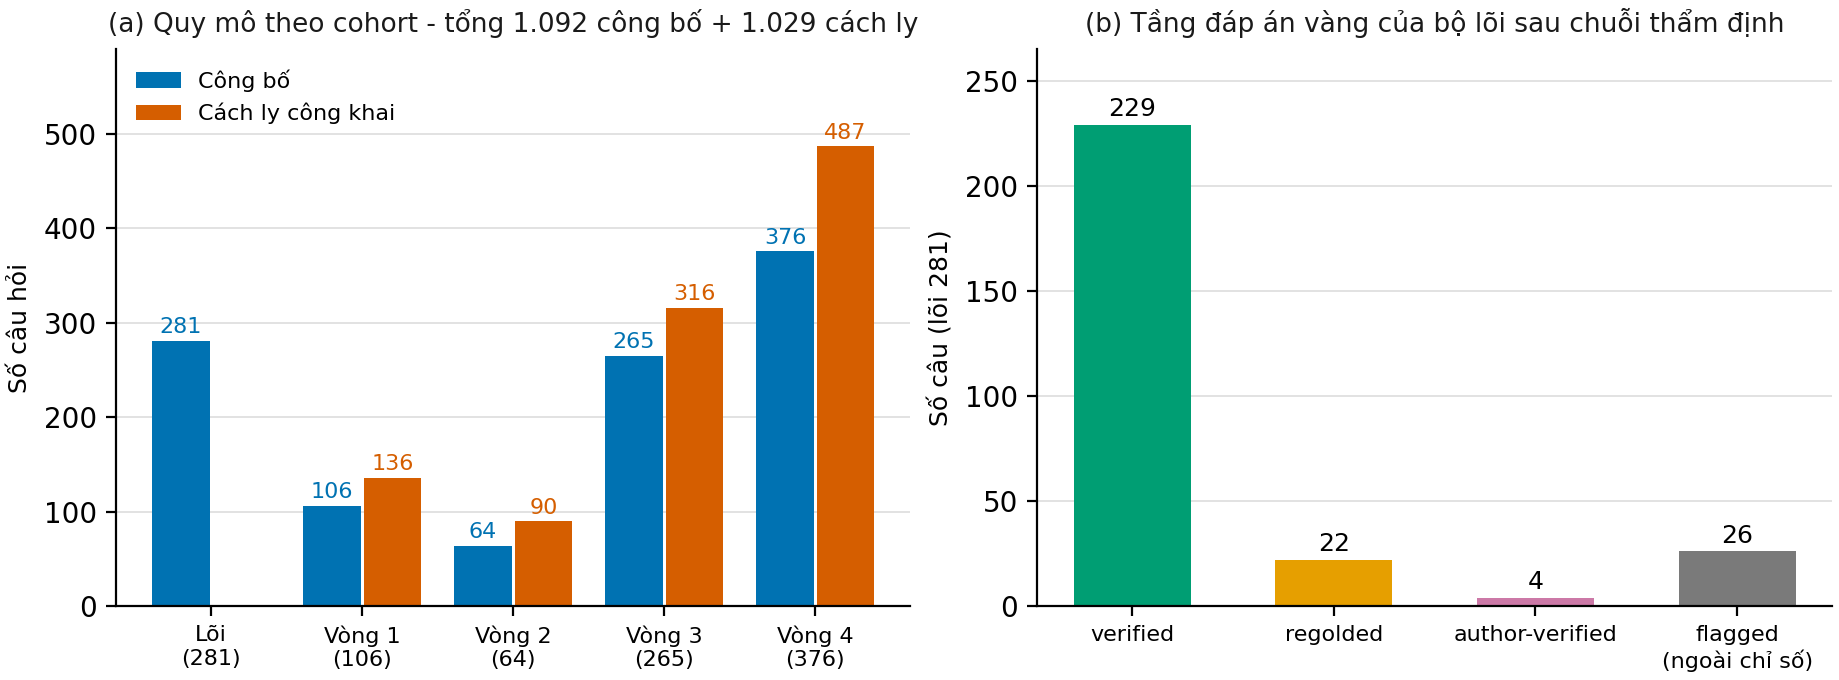
\includegraphics[width=\linewidth]{figures/fig_composition.png}
\caption{Cấu trúc ViCivil-TKG: năm cohort công bố kèm tầng chất lượng vàng và phần cách ly công khai. Các câu cách ly không bao giờ được tính vào chỉ số.}
\label{fig:composition}
\end{figure}

\section{Thiết lập thực nghiệm}

\textbf{Truy hồi.} Giao thức hợp nhất: BM25 (Python thuần, $k_1{=}1{,}2$, $b{=}0{,}75$) + dense 768 chiều (vector đoạn đã lưu, \texttt{embeddinggemma:300m}) hợp nhất bằng RRF $k{=}60$, lấy 200 ứng viên mỗi nhánh. Chấm điểm đối chiếu định danh đoạn vàng chính xác; báo cáo Hit@\{1,3,5,10\} và MRR. TCR (temporal-consistency retrieval) lọc ứng viên theo cửa sổ hiệu lực của văn bản tại \texttt{as\_of} của câu hỏi; văn bản ngoài đồ thị được giữ nguyên. Với cohort mở rộng, thêm điều kiện xếp hạng lại BGE-reranker-v2-m3 trên 30 ứng viên rồi áp TCR. Ý nghĩa thống kê: Wilcoxon cặp trên nghịch đảo hạng của lần trúng vàng đầu tiên. Semantics của MRR được ghi chú riêng cho từng bảng: MRR danh sách đầy đủ cho kết quả lõi có TCR, MRR@10 cho lần chạy lại không TCR (giao thức chấm lại theo cửa sổ), và MRR@30 cho các bảng hiệu ứng vàng và rerank (cửa sổ 30 ứng viên) - không so chéo giữa các semantics.

\textbf{Sinh có trích dẫn.} Qwen2.5-3B-Instruct (greedy, tối đa 180 token mới, batch 6) chạy trên bốn điều kiện: \emph{norag} (không ngữ cảnh), \emph{rag\_hybrid} (top-5 truy hồi hợp nhất), \emph{rag\_hybrid\_tcr} (top-5 sau TCR), \emph{rag\_rerank\_tcr} (top-5 sau rerank + TCR). Đo \emph{cite\_acc} (câu trả lời có nêu đúng điều luật trong tập vàng), \emph{span\_F1} (F1 token với văn bản vàng), \emph{abstain} (tỷ lệ trả lời ``Không đủ thông tin''), \emph{ctx\_hit5} (tập vàng xuất hiện trong ngữ cảnh). Ý nghĩa thống kê: McNemar chính xác cho cite\_acc, Wilcoxon cho span\_F1.

\textbf{Tái lập.} Toàn bộ chỉ số truy hồi và chấm lại LLM đều tính từ các artefact đã lưu (vector, xếp hạng, câu trả lời), chạy được bằng \texttt{tools/reproduce.sh} mà không cần GPU hay truy cập mạng.

\section{Kết quả}

\subsection{Truy hồi trên bộ lõi}

Bảng~\ref{tab:core-retrieval} báo cáo kết quả trên 281 câu lõi với giao thức hybrid+TCR đã tài liệu hoá. Điểm tổng thể đạt Hit@5 0,811 và MRR 0,662 (chấm lại toàn danh sách sau khi persist pass-3; bảng suite so sánh 4 hệ thống dùng cửa sổ ứng viên top-200 nên MRR là 0,660 - cả hai snapshot đều được công bố, không thay thế im lặng); trên tầng vàng \texttt{verified} (229 câu) đạt Hit@5 0,821 và MRR 0,693. Ba tầng vàng thấp hơn - \texttt{flagged} (26 câu, Hit@5 0,692), \texttt{regolded} (22 câu, Hit@1 chỉ 0,273 nhưng Hit@5 0,864), \texttt{author-verified} (4 câu) - được công bố nguyên vẹn: pattern ``Hit@1 thấp, Hit@5 cao'' của tầng regolded cho thấy các đoạn được neo lại thường nằm sâu trong danh sách ứng viên, đúng loại trường hợp mà không có thẩm định đa vòng sẽ bị tính là trượt. Lần chạy lại không TCR (cùng mã chấm, bỏ lọc thời hiệu) đạt Hit@5 0,733 so với 0,811: khoảng cách này chính là đóng góp của lọc thời hiệu, và mức tăng tái lập trên cả bốn cohort mở rộng (Hình~\ref{fig:hitk}).

Bảng~\ref{tab:baselines-vn} mở rộng phép so sánh sang hai tín hiệu đơn lẻ trên cùng một harness tính lại trực tiếp từ ảnh kho đã phát hành. Hai nhận định nổi bật. Thứ nhất, không tín hiệu đơn lẻ nào vượt trội: trên bộ lõi, dense so với BM25 khác biệt không có ý nghĩa thống kê (Wilcoxon $p=0{,}257$; trên toàn bộ 1.092 câu $p=0{,}213$), trong khi phép hợp nhất thì có (hybrid so với dense $p=1{,}8\times10^{-4}$; hybrid so với BM25 $p=7{,}9\times10^{-8}$). Thứ hai, lọc thời hiệu là yếu tố đơn lớn nhất ở mọi nơi: hybrid+TCR so với hybrid cho $p=8{,}5\times10^{-23}$ trên lõi và $p=2{,}6\times10^{-66}$ trên toàn bộ 1.092 câu công bố.

\begin{table}[t]
\centering\small
\caption{Suite baseline trên bộ lõi 281 câu và toàn bộ 1.092 câu công bố, một harness thống nhất tính lại tươi (BM25 $k_1{=}1{,}2$, $b{=}0{,}75$; dense 768 chiều; RRF $k{=}60$; TCR = lọc cửa sổ hiệu lực). MRR tính trong cửa sổ ứng viên.}
\label{tab:baselines-vn}
\setlength{\tabcolsep}{3.4pt}
\begin{tabular}{l ccc ccc}
\toprule
 & \multicolumn{3}{c}{Lõi (281)} & \multicolumn{3}{c}{Toàn bộ (1.092)} \\
\cmidrule(lr){2-4}\cmidrule(lr){5-7}
Hệ thống & Hit@1 & Hit@5 & MRR & Hit@1 & Hit@5 & MRR \\
\midrule
BM25 thuần & 0,331 & 0,644 & 0,472 & 0,424 & 0,730 & 0,562 \\
Dense thuần & 0,356 & 0,666 & 0,495 & 0,430 & 0,761 & 0,575 \\
Hybrid (RRF) & 0,399 & 0,733 & 0,546 & 0,469 & 0,809 & 0,617 \\
Hybrid + TCR & \textbf{0,537} & \textbf{0,811} & \textbf{0,660} & \textbf{0,608} & \textbf{0,863} & \textbf{0,721} \\
\bottomrule
\end{tabular}

\smallskip
{\footnotesize Wilcoxon cặp trên lõi: TCR so với hybrid $p=8{,}5\times10^{-23}$; hybrid so với dense $p=1{,}8\times10^{-4}$; hybrid so với BM25 $p=7{,}9\times10^{-8}$; dense so với BM25 $p=0{,}257$ (không có ý nghĩa thống kê). Trên toàn bộ 1.092 câu: TCR so với hybrid $p=2{,}6\times10^{-66}$; dense so với BM25 $p=0{,}213$ (không có ý nghĩa).}
\end{table}

\begin{table}[t]
\centering\small
\caption{Truy hồi trên bộ lõi 281 câu (hybrid BM25+dense+RRF, lọc thời hiệu TCR; MRR danh sách đầy đủ, hàng cuối MRR@10).}
\label{tab:core-retrieval}
\setlength{\tabcolsep}{3.6pt}
\begin{tabular}{lrrrrrr}
\toprule
Nhóm & $n$ & Hit@1 & Hit@3 & Hit@5 & Hit@10 & MRR \\
\midrule
Toàn bộ & 281 & \textbf{0,541} & \textbf{0,740} & \textbf{0,811} & \textbf{0,879} & \textbf{0,662} \\
\quad verified & 229 & 0,585 & 0,760 & 0,821 & 0,895 & 0,693 \\
\quad regolded & 22 & 0,273 & 0,773 & 0,864 & 0,909 & 0,532 \\
\quad author-verified & 4 & 0,250 & 0,500 & 0,750 & 0,750 & 0,403 \\
\quad flagged (không tính điểm chính) & 26 & 0,423 & 0,577 & 0,692 & 0,731 & 0,538 \\
\midrule
Chạy lại không TCR (MRR@10) & 281 & 0,399 & 0,651 & 0,733 & 0,815 & 0,540 \\
\bottomrule
\end{tabular}
\end{table}

\begin{figure}[t]
\centering
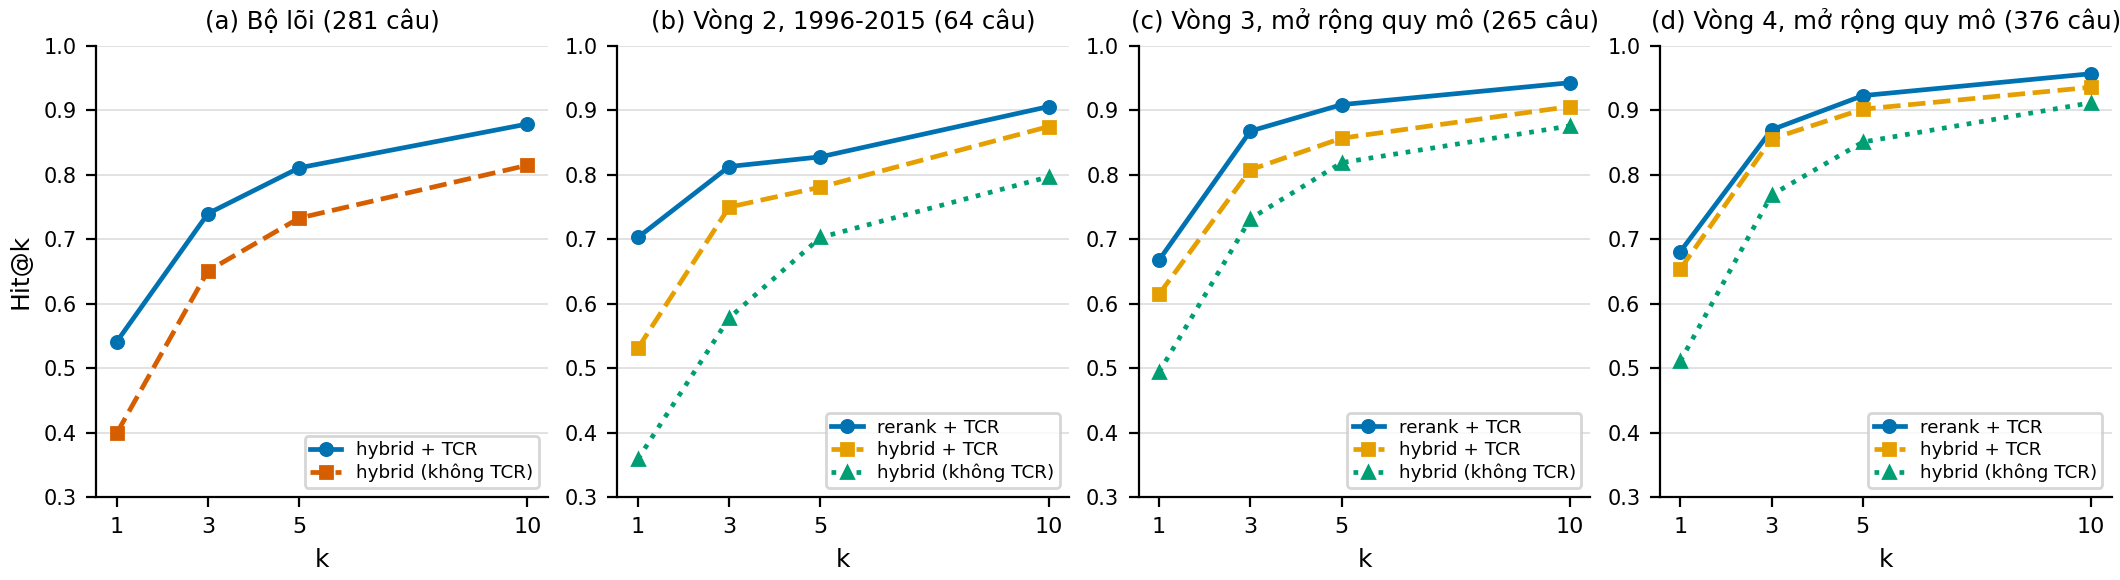
\includegraphics[width=\linewidth]{figures/fig_hitk.png}
\caption{Đường Hit@k trên cùng một harness truy hồi: (a) bộ lõi có và không lọc thời hiệu; (b) cohort 1996-2015; (c) vòng~3 và (d) vòng~4 mở rộng quy mô. Mọi đường đều dùng chung vector đoạn đã lưu và mã hợp nhất RRF; khoảng cách giữa các đường chính là đóng góp cộng dồn của xếp hạng lại và lọc thời hiệu.}
\label{fig:hitk}
\end{figure}

\subsection{Hiệu ứng của chuỗi thẩm định vàng}

Bảng~\ref{tab:gold-effect} tách hai đại lượng bị trộn lẫn trong phiên bản phát hành đầu tiên. \emph{Hiệu ứng áp dụng} là chênh lệch giữa vàng trong tệp câu hỏi trước và sau khi persist neo lại pass-3 của TOP27031 (lỗi B1, Mục~\ref{sec:audit}): Hit@5 danh sách rerank đổi 0,794$\rightarrow$0,797, MRR 0,5957$\rightarrow$0,5964; Hit@1 danh sách hybrid 0,406$\rightarrow$0,409. \emph{Hàng phân tích độ nhạy} chấm cùng danh sách ứng viên đã lưu với 24 tập vàng ``đã ghi nhưng không bao giờ áp dụng'' (18 tập tương đương phiên bản + 6 đề xuất neo lại, trong đó 1 bị guardrail chặn): Hit@1 0,484 và MRR 0,621 trên danh sách rerank. Hàng này chỉ là phân tích độ nhạy theo độ rộng tập vàng và \emph{không phải chỉ số chính} - mọi số chính trong báo cáo đều chấm trên vàng đã áp dụng. Thông điệp của bảng là chất lượng neo vàng trở thành đại lượng đo được theo từng tầng, và việc tách bạch hai loại số giữ cho bảng không bị đọc sai thành mức tăng ``miễn phí''.

\begin{table}[t]
\centering\small
\caption{Hiệu ứng tập vàng và phân tích độ nhạy trên bộ lõi: cùng danh sách ứng viên đã lưu (rerank / hybrid, 30 ứng viên, MRR@30), chấm với các tập vàng khác nhau (281 câu).}
\label{tab:gold-effect}
\begin{tabular}{lcccccc}
\toprule
 & \multicolumn{3}{c}{Danh sách rerank} & \multicolumn{3}{c}{Danh sách hybrid} \\
\cmidrule(lr){2-4}\cmidrule(lr){5-7}
Tập vàng & Hit@1 & Hit@5 & MRR & Hit@1 & Hit@5 & MRR \\
\midrule
Đã áp dụng: trước persist & 0,448 & 0,794 & 0,596 & 0,406 & 0,737 & 0,548 \\
Đã áp dụng: sau persist & 0,448 & \textbf{0,797} & \textbf{0,596} & \textbf{0,409} & \textbf{0,740} & \textbf{0,552} \\
\midrule
24 đã ghi, không áp dụng (độ nhạy) & 0,484 & 0,808 & 0,621 & 0,441 & 0,744 & 0,571 \\
\bottomrule
\end{tabular}
\end{table}

\subsection{Sinh có trích dẫn trên bộ lõi}

Bảng~\ref{tab:core-llm} và Hình~\ref{fig:llm} trình bày bốn điều kiện. Không có ngữ cảnh, mô hình gần như không bao giờ nêu đúng điều luật (cite\_acc 0,004) và từ chối trả lời 54,8\% số câu. Cung cấp ngữ cảnh hợp nhất đưa cite\_acc lên 0,488; lọc thời hiệu đẩy lên \textbf{0,601} (+0,114 điểm tuyệt đối, McNemar $p=5{,}8\times10^{-5}$; mọi cặp so sánh với no-RAG đạt $p<10^{-40}$). Rerank+TCR nâng cite\_acc lên 0,604 (McNemar $p=7{,}3\times10^{-4}$ so với hybrid) và ctx\_hit5 lên 0,850. Các giá trị ctx\_hit5 được tính lại trong kiểm toán toàn vẹn đối chiếu với vàng đã áp dụng từ danh sách ngữ cảnh top-5 đã lưu (trước đó giữ giá trị runtime ghi trước chuỗi regold - lỗi B5); lần tính lại (208/281 $=$ 0,740; 229/281 $=$ 0,815; 238/280 $=$ 0,850) khớp với Hit@5 truy hồi của cấu hình tương ứng, và giá trị runtime cũ được giữ nguyên trong artefact phát hành dưới tên \texttt{ctx\_hit5\_runtime\_pre\_pass\_3}. Hai điểm yếu được công bố thẳng: một câu (NEW90253) bị loại khỏi điều kiện rerank+TCR vì bể ứng viên cạn sau lọc thời hiệu ($n{=}280$); câu trả lời được lưu nguyên văn, thỉnh thoảng lẫn ký tự CJK do mô hình 3B sinh ra (11/281 ở no-RAG, $\le$5/281 ở các nhánh RAG) - không can thiệp làm sạch sau khi thu thập. Tỷ lệ từ chối giữ ổn định quanh 11\% khi có ngữ cảnh - mô hình hiếm khi ``nói bừa'' khi trích dẫn không đủ, hợp lý với thiết kế prompt.

\begin{table}[t]
\centering\small
\caption{Sinh có trích dẫn trên bộ lõi (Qwen2.5-3B-Instruct, greedy, 180 token; ctx\_hit5 chấm trên vàng đã áp dụng).}
\label{tab:core-llm}
\begin{tabular}{lccccc}
\toprule
Điều kiện & cite\_acc & span\_F1 & abstain & ctx\_hit5 & $n$ \\
\midrule
No-RAG & 0,004 & 0,324 & 0,548 & - & 281 \\
RAG hybrid & 0,488 & 0,465 & 0,110 & 0,740 & 281 \\
RAG hybrid + TCR & \textbf{0,601} & 0,489 & 0,107 & 0,815 & 281 \\
RAG rerank + TCR & \textbf{0,604} & \textbf{0,490} & 0,111 & \textbf{0,850} & 280 \\
\bottomrule
\end{tabular}
\end{table}

\begin{figure}[t]
\centering
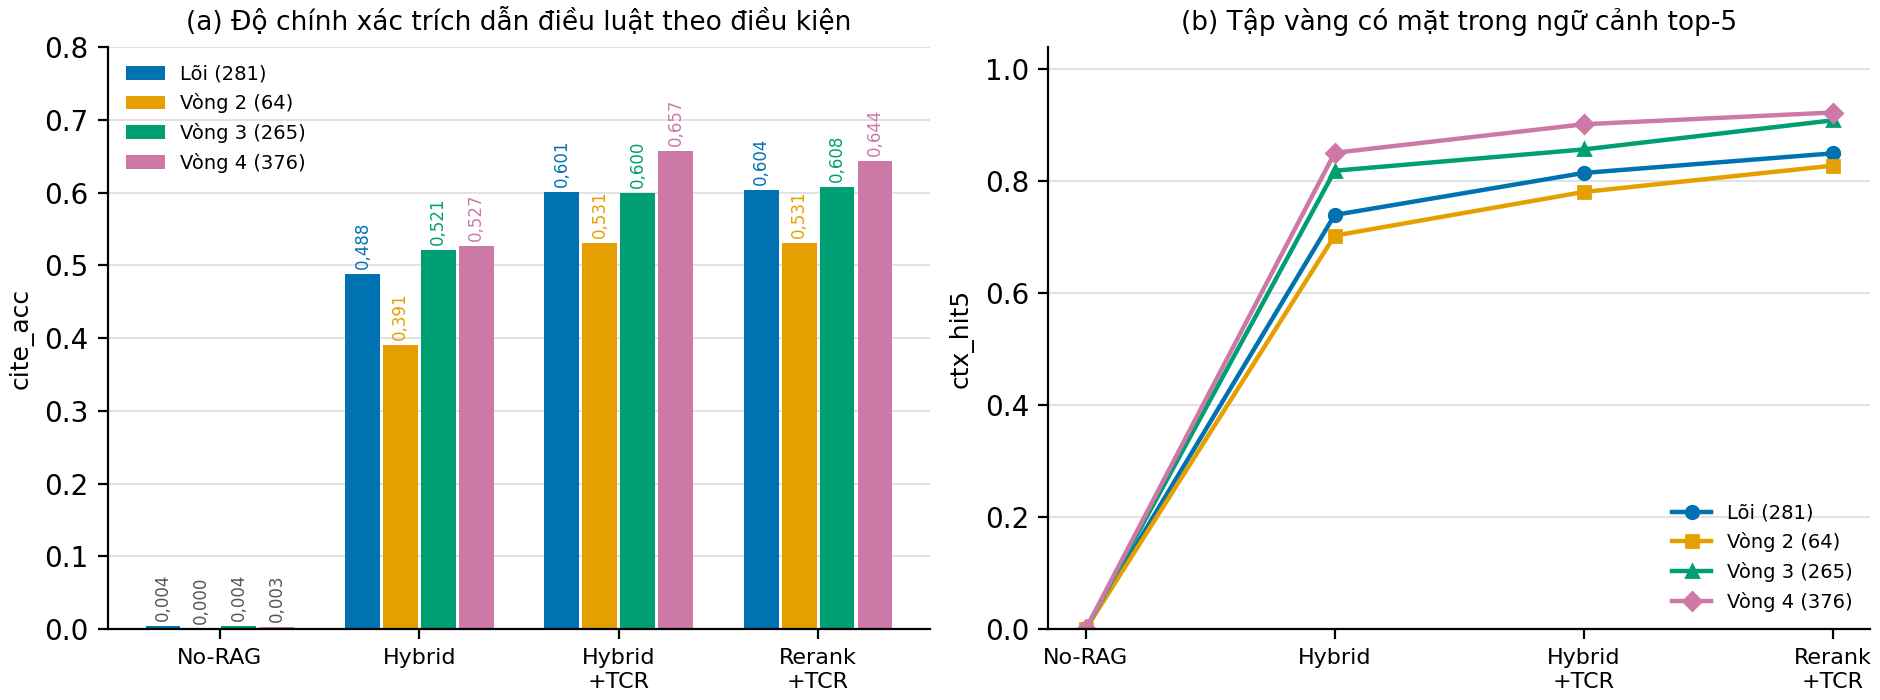
\includegraphics[width=\linewidth]{figures/fig_llm_conditions.png}
\caption{cite\_acc (a) và ctx\_hit5 (b) theo bốn điều kiện trên bộ lõi 281 câu và ba cohort mở rộng có bài sinh (vòng~2: 64, vòng~3: 265, vòng~4: 376 câu). Khoảng cách giữa cột cite\_acc và đường ctx\_hit5 cùng màu là dư địa còn lại ở bước sinh trong mọi cohort; hiệu ứng thời hiệu mạnh nhất ở vòng~4 (0,527$\rightarrow$0,657).}
\label{fig:llm}
\end{figure}

\subsection{Cohort mở rộng: vòng 1-4}

Bảng~\ref{tab:ext} tổng hợp cả bốn cohort mở rộng và Hình~\ref{fig:hitk} vẽ đường Hit@k tương ứng. Trên vòng~1 (106 câu), TCR nâng Hit@1 từ 0,547 lên 0,689 và Hit@5 từ 0,906 lên 0,925 (Wilcoxon $p=2{,}1\times10^{-5}$); riêng rerank thuần không có ý nghĩa ($p=0{,}42$) và rerank+TCR ở mức 0,651 cũng chưa ($p=0{,}71$ so với TCR) - công bố nguyên trạng. Trên vòng~2 - văn bản 1996-2015 hiếm và cũ hơn - mọi chỉ số giảm rõ: TCR nâng Hit@5 từ 0,703 lên 0,781 và MRR@30 từ 0,517 lên 0,648 ($p=4{,}0\times10^{-5}$); rerank+TCR đạt Hit@1 \textbf{0,703} ($p=1{,}4\times10^{-3}$ so với TCR). Tầng \texttt{regolded} của vòng~2 (11 câu) là lát cắt khó nhất toàn bộ bộ chuẩn (Hit@1 0,091, Hit@5 0,364) - hệ quả trực tiếp của việc neo vàng trên văn bản cũ, được ghi nhãn công khai để người dùng stratify. Vòng~3 (265 câu trên 19 văn bản) mang tính chất trung gian: TCR nâng Hit@1 0,494$\rightarrow$0,615 và Hit@5 0,819$\rightarrow$0,857 ($p=5{,}7\times10^{-17}$); rerank+TCR đạt Hit@1 \textbf{0,668} và Hit@5 \textbf{0,909} ($p=5{,}2\times10^{-3}$ so với TCR - cohort đầu tiên mà rerank cộng thêm mức tăng có ý nghĩa trên nền TCR). Vòng~4 (376 câu, cohort lớn nhất) xác nhận quy luật trên quy mô mới: TCR nâng Hit@1 0,511$\rightarrow$0,654 và Hit@5 0,851$\rightarrow$0,902 ($p=6{,}3\times10^{-22}$); rerank+TCR đạt Hit@1 \textbf{0,681} và Hit@5 \textbf{0,923}, dù mức tăng thêm so với TCR thuần chưa qua ngưỡng ý nghĩa trên cohort này ($p=0{,}10$, công bố nguyên trạng). Tầng \texttt{regolded} vòng~4 (13 câu) lặp lại chữ ký Hit@1 thấp (0,231), và - khác bốn neo vòng~2 nêu ở Mục~6 - \emph{tất cả} neo regolded vòng~4 nằm trong cửa sổ hiệu lực tại \texttt{as\_of} của câu hỏi.

Sinh có trích dẫn chạy đồng bộ trên cả ba cohort có bài sinh (vòng~2, vòng~3, vòng~4) đúng giao thức của Bảng~\ref{tab:core-llm}. Trên vòng~2, chuỗi cải thiện xuất hiện trọn vẹn (0,000$\rightarrow$0,531 cite\_acc sau lọc thời hiệu; McNemar $p=1{,}2\times10^{-10}$ so với không ngữ cảnh), dù span\_F1 của rerank+TCR vượt TCR thuần mà chưa qua ngưỡng ý nghĩa (Wilcoxon $p=0{,}083$) - chúng tôi báo cáo nguyên trạng, không khẳng định quá mức. Vòng~3 (Bảng~\ref{tab:ext3-llm}): cite\_acc tăng từ 0,004 không ngữ cảnh lên 0,521 với ngữ cảnh hợp nhất và \textbf{0,600} sau lọc thời hiệu (McNemar $p=3{,}8\times10^{-3}$ so với hybrid), 0,608 với rerank+TCR - chưa có ý nghĩa so với TCR ($p=0{,}89$), đối lập với phía truy hồi nơi rerank+TCR có ý nghĩa ($p=5{,}2\times10^{-3}$); ctx\_hit5 từng cấu hình trùng khớp chính xác Hit@5 truy hồi (0,819 / 0,857 / 0,909) - nhất quán chéo pipeline như ở bộ lõi; tỷ lệ từ chối giảm từ 46,0\% xuống 15-20\% khi có ngữ cảnh. Vòng~4 cho hiệu ứng thời hiệu mạnh nhất mọi cohort (Bảng~\ref{tab:ext4-llm}): cite\_acc 0,003 (không ngữ cảnh) $\rightarrow$ 0,527 (hybrid) $\rightarrow$ \textbf{0,657} sau lọc thời hiệu - mức tăng tuyệt đối +0,130 (McNemar $p=3{,}2\times10^{-10}$) - với rerank+TCR ở mức 0,644, không phân biệt được thống kê với TCR ($p=0{,}635$); ctx\_hit5 lại trùng Hit@5 truy hồi (0,851 / 0,902 / 0,923).

\begin{table}[t]
\centering\footnotesize
\caption{Cohort mở rộng: tỉ lệ trúng truy hồi và phép thử Wilcoxon cặp.}
\label{tab:ext}
\setlength{\tabcolsep}{3.0pt}
\begin{tabular}{lcccccccc}
\toprule
 & \multicolumn{2}{c}{V1 ($n{=}106$)} & \multicolumn{2}{c}{V2 1996-2015 ($n{=}64$)} & \multicolumn{2}{c}{V3 ($n{=}265$)} & \multicolumn{2}{c}{V4 ($n{=}376$)} \\
\cmidrule(lr){2-3}\cmidrule(lr){4-5}\cmidrule(lr){6-7}\cmidrule(lr){8-9}
Cấu hình & Hit@1 & Hit@5 & Hit@1 & Hit@5 & Hit@1 & Hit@5 & Hit@1 & Hit@5 \\
\midrule
Hybrid (base) & 0,547 & 0,906 & 0,359 & 0,703 & 0,494 & 0,819 & 0,511 & 0,851 \\
Hybrid + TCR & \textbf{0,689} & \textbf{0,925} & 0,531 & 0,781 & 0,615 & 0,857 & 0,654 & 0,902 \\
Rerank & 0,585 & 0,906 & 0,516 & 0,797 & 0,555 & 0,879 & 0,588 & 0,875 \\
Rerank + TCR & 0,651 & 0,943 & \textbf{0,703} & \textbf{0,828} & \textbf{0,668} & \textbf{0,909} & \textbf{0,681} & \textbf{0,923} \\
\bottomrule
\end{tabular}

\vspace{3pt}
{\footnotesize MRR@30 theo hàng (base / +TCR / rerank / rerank+TCR): vòng~1 - 0,700 / 0,790 / 0,726 / 0,779; vòng~2 - 0,517 / 0,648 / 0,654 / 0,766; vòng~3 - 0,629 / 0,724 / 0,694 / 0,775; vòng~4 - 0,660 / 0,763 / 0,716 / 0,787. $p$ (TCR so với base): $2{,}1\times10^{-5}$, $4{,}0\times10^{-5}$, $5{,}7\times10^{-17}$, $6{,}3\times10^{-22}$; $p$ (rerank+TCR so với TCR): 0,71 (v1, không có ý nghĩa), $1{,}4\times10^{-3}$ (v2), $5{,}2\times10^{-3}$ (v3), 0,10 (v4, không có ý nghĩa).}
\end{table}

\begin{table}[t]
\centering\small
\caption{Sinh có trích dẫn trên vòng~3 (265 câu; Qwen2.5-3B-Instruct, greedy, 180 token - đúng giao thức Bảng~\ref{tab:core-llm}).}
\label{tab:ext3-llm}
\setlength{\tabcolsep}{3.6pt}
\begin{tabular}{lccccc}
\toprule
Điều kiện & cite\_acc & span\_F1 & abstain & ctx\_hit5 & $n$ \\
\midrule
No-RAG & 0,004 & 0,338 & 0,460 & - & 265 \\
RAG hybrid & 0,521 & 0,444 & 0,196 & 0,819 & 265 \\
RAG hybrid + TCR & \textbf{0,600} & \textbf{0,475} & 0,155 & 0,857 & 265 \\
RAG rerank + TCR & \textbf{0,608} & 0,470 & \textbf{0,151} & \textbf{0,909} & 265 \\
\bottomrule
\end{tabular}

\vspace{3pt}
{\footnotesize McNemar trên cite\_acc: +TCR so với hybrid $p=3{,}8\times10^{-3}$; rerank+TCR so với TCR $p=0{,}89$ (không có ý nghĩa); no-RAG so với hybrid+TCR $p=5{,}5\times10^{-48}$. Wilcoxon trên span\_F1: +TCR so với hybrid $p=1{,}5\times10^{-4}$.}
\end{table}

\begin{table}[t]
\centering\small
\caption{Sinh có trích dẫn trên vòng~4 (376 câu; cùng giao thức).}
\label{tab:ext4-llm}
\setlength{\tabcolsep}{3.6pt}
\begin{tabular}{lccccc}
\toprule
Điều kiện & cite\_acc & span\_F1 & abstain & ctx\_hit5 & $n$ \\
\midrule
No-RAG & 0,003 & 0,339 & 0,465 & - & 376 \\
RAG hybrid & 0,527 & 0,468 & 0,168 & 0,851 & 376 \\
RAG hybrid + TCR & \textbf{0,657} & \textbf{0,502} & 0,144 & 0,902 & 376 \\
RAG rerank + TCR & 0,644 & 0,493 & \textbf{0,141} & \textbf{0,923} & 376 \\
\bottomrule
\end{tabular}

\vspace{3pt}
{\footnotesize McNemar trên cite\_acc: +TCR so với hybrid $p=3{,}2\times10^{-10}$; rerank+TCR so với TCR $p=0{,}635$ (không có ý nghĩa); no-RAG so với hybrid+TCR $p=1{,}8\times10^{-74}$. Wilcoxon trên span\_F1: +TCR so với hybrid $p=1{,}0\times10^{-7}$.}
\end{table}

\subsection{Thống kê tổng hợp}

Mọi so sánh chính đều kèm phép thử cặp; các so sánh không đạt ngưỡng được ghi rõ là không có ý nghĩa thay vì bỏ đi: (i) truy hồi, TCR so với base: $p=2{,}1\times10^{-5}$ (vòng~1), $p=4{,}0\times10^{-5}$ (vòng~2), $p=5{,}7\times10^{-17}$ (vòng~3), $p=6{,}3\times10^{-22}$ (vòng~4), $p=2{,}6\times10^{-66}$ (toàn bộ 1.092 câu); (ii) rerank+TCR so với TCR: $p=1{,}4\times10^{-3}$ (vòng~2), $p=5{,}2\times10^{-3}$ (vòng~3), $p=0{,}10$ (vòng~4, không có ý nghĩa); (iii) sinh, hybrid+TCR so với hybrid: McNemar $p=5{,}8\times10^{-5}$ (lõi), $p=0{,}012$ (vòng~2); no-RAG so với hybrid+TCR: $p<10^{-40}$ trên các cohort có bài sinh; (iv) sinh vòng~3: $p=3{,}8\times10^{-3}$ (+TCR so với hybrid), rerank+TCR so với TCR $p=0{,}89$ (không có ý nghĩa), no-RAG so với hybrid+TCR $p=5{,}5\times10^{-48}$; (v) sinh vòng~4: $p=3{,}2\times10^{-10}$, rerank+TCR so với TCR $p=0{,}635$ (không có ý nghĩa), no-RAG so với hybrid+TCR $p=1{,}8\times10^{-74}$. Các so sánh span\_F1 khi không đạt ngưỡng được ghi rõ là không có ý nghĩa.

\subsection{Kiểm toán toàn vẹn dữ liệu và tái lập}
\label{sec:audit}

Trước khi đóng băng phát hành, chúng tôi chạy kiểm toán toàn vẹn trên toàn bộ artefact công bố theo quy tắc \emph{chạy lại rồi mới vá}: mỗi chỉ số được tính lại độc lập từ artefact per-question, và chỉ vá sau khi lần tính lại khớp số đã công bố tới bốn chữ số thập phân. Kiểm toán xác nhận khớp chính xác EXT1/EXT2, các ô tái lập và hiệu ứng vàng, cùng kích thước cohort bằng đếm trực tiếp. Ba lỗi dữ liệu thực sự được phát hiện và sửa kèm nhật ký (\texttt{CHANGES.json}, 30 thay đổi): (B1) neo lại pass-3 của TOP27031 được ghi nhận nhưng không bao giờ được persist vào tệp câu hỏi (vàng cũ ở hạng 31, vàng đúng ở hạng 1) - đã persist, tầng đổi từ flagged sang regolded, mọi chỉ số lõi được tính lại trên vàng đã áp dụng; (B2) \texttt{gold\_adjudicated.json} trộn 24 tập vàng ``đã ghi nhưng không áp dụng'' vào bản đồ áp dụng - tách riêng vào \texttt{proposals\_not\_applied}; (B3) kit thẩm định người thiếu \texttt{as\_of} ở 50/60 dòng và mang vàng cũ ở 7/60 dòng - kit được tạo lại đồng bộ với vàng đã áp dụng. Ngoài ra ctx\_hit5 được tính lại (lỗi giá trị cũ B5) và đối chiếu khớp chính xác với Hit@5 truy hồi từng cấu hình. Sau khi vá: Hit@5 lõi 0,808$\rightarrow$0,811, MRR 0,659$\rightarrow$0,662, cite\_acc TCR giữ nguyên 0,601; EXT1/EXT2 không đổi. Toàn bộ quy trình, số cũ$\rightarrow$mới và bảng băm SHA-256 mới được công bố trong \texttt{AUDIT\_2026-11-01.md} - chúng tôi cho rằng kiểu kiểm toán này nên là bắt buộc với mọi benchmark công khai trước khi nộp bài.

\section{Thảo luận và hạn chế}

\textbf{Hạn chế của dữ liệu.} (1) Miền hẹp: toàn bộ câu hỏi thuộc luật dân sự - tố tụng dân sự; 20 văn bản và 1.092 câu vẫn nhỏ so với các benchmark đa miền. (2) Tầng vàng không đồng nhất: 26 câu lõi bị cờ và được loại khỏi chỉ số chính; tầng regolded (22 câu) có Hit@1 thấp một cách có hệ thống - người dùng bộ chuẩn cần stratify theo tầng như chúng tôi đã làm. (3) Thỏa thuận giữa thẩm định viên độc lập chỉ đạt 0,554 trên mẫu 60 câu; đây là kiểm tra giữa các mô hình trên tác vụ chọn đoạn trong 8 ứng viên - nhiệm vụ vốn nhiều ứng viên đúng - và \emph{không thay thế được} đánh giá con người. Kit thẩm định người đã sẵn sàng sử dụng ngay: bảng 60 câu phân tầng, ba packet độc lập cho ba thẩm định viên (xáo trộn với seed cố định riêng; mỗi packet chỉ hiển thị cột chấm của người đó để bảo đảm tính độc lập), rubric DUNG/SAI/MỘT PHẦN kèm hướng dẫn, và fixture kiểm thử có nhãn rõ \emph{TEST-ONLY} trên đó triển khai Cohen/Fleiss $\kappa$ tái lập chính xác giá trị tham chiếu tính tay; chỉ còn bước chạy với thẩm định viên người thật trước khi công bố $\kappa$. (4) Câu hỏi sinh từ LLM, do đó mang thiên lệch của mô hình sinh; chúng tôi giảm nhẹ bằng dedup vector, audit hai tầng và cách ly công khai, nhưng không loại trừ hoàn toàn. (5) Bốn neo \texttt{regolded} vòng~2 (EXT20028, EXT20039, EXT20113, EXT20123 - 4/11) nằm ngoài phạm vi thời hiệu tại \texttt{as\_of} của câu hỏi: ba neo đầu trỏ tới văn bản hợp nhất có cửa sổ hiệu lực bắt đầu \emph{sau} \texttt{as\_of}, còn EXT20123 trỏ tới đoạn BLDS~1995 đã hết hiệu lực từ 01-01-2006, trước \texttt{as\_of} của nó sáu năm. Mỗi neo đều được chuỗi thẩm định chấp nhận là cơ sở pháp lý của câu hỏi gốc, nhưng cả bốn rơi ngoài cửa sổ hiệu lực tại ngày ghi, nên lọc TCR phạt chúng theo cấu tạo; chúng tôi công bố thay vì neo lại lần thứ hai im lặng, và chúng góp phần vào số liệu thấp của tầng regolded nêu trên.

\textbf{Hạn chế của đánh giá.} Các thí nghiệm dùng một mô hình sinh 3B và một reranker; chưa có baseline LLM lớn hơn hay fine-tune trên miền. TCR dựa trên đồ thị thời gian thủ công xác nhận; sai sót trong cửa sổ hiệu lực sẽ truyền trực tiếp vào lọc. Ba semantics MRR (danh sách đầy đủ / MRR@10 / MRR@30) được chú thích riêng từng bảng nhưng chưa thống nhất - chuẩn hoá về danh sách đầy đủ là việc kỹ thuật tiếp theo. Chỉ số cite\_acc đo việc nêu đúng \emph{số} điều luật, chưa đo việc trích đúng \emph{đoạn}.

\textbf{Đạo đức và mục đích sử dụng.} Toàn bộ kho văn bản là các văn bản pháp luật công khai với provenance từng đoạn và nhãn loại nguồn; không có dữ liệu cá nhân. Bộ chuẩn dùng để đánh giá hệ thống truy hồi và hỏi-đáp trên văn bản luật Việt Nam; câu trả lời do mô hình sinh ra khi được đánh giá trên bộ chuẩn này không phải là tư vấn pháp lý.

\section{Kết luận}

ViCivil-TKG cho thấy hai nguyên tắc - kiểm định thời hiệu và thẩm định vàng đa tầng với cách ly công khai - có thể được vận hành nhất quán trên dữ liệu pháp lý tiếng Việt, và cả hai đều cho hiệu quả đo được: TCR cải thiện cite\_acc +0,114 điểm ($p<10^{-4}$) và Hit@5 truy hồi trên mọi cohort; chuỗi thẩm định loại bỏ hoàn toàn trạng thái vàng không xác minh được và làm cho chất lượng neo vàng đo được theo từng tầng. Đóng góp phương pháp luận thứ ba là quy trình kiểm toán \emph{chạy lại rồi mới vá} với nhật ký thay đổi công khai đầy đủ. Bộ chuẩn 1.092 câu kèm 1.029 câu cách ly, dấu vết provenance đầy đủ, kit thẩm định người và kịch bản tái lập không GPU được công bố để cộng đồng kiểm chứng và mở rộng; hướng tiếp theo ưu tiên là thẩm định con người trên mẫu phân tầng (kit đã sẵn sàng), thống nhất semantics MRR, mở rộng sang văn bản cấp thông tư và các miền luật lân cận, và benchmark các mô hình sinh lớn hơn.

\begin{thebibliography}{9}\small

\bibitem{robertson2009bm25} S. Robertson, H. Zaragoza, ``The Probabilistic Relevance Framework: BM25 and Beyond,'' \emph{Foundations and Trends in Information Retrieval}, 3(4), 2009.

\bibitem{cormack2009rrf} G. V. Cormack, C. L. A. Clarke, S. B\"uttcher, ``Reciprocal Rank Fusion Outperforms Condorcet and Individual Rank Learning Methods,'' \emph{SIGIR}, 2009.

\bibitem{karpukhin2020dpr} V. Karpukhin \emph{et al.}, ``Dense Passage Retrieval for Open-Domain Question Answering,'' \emph{EMNLP}, 2020.

\bibitem{thakur2021beir} N. Thakur \emph{et al.}, ``BEIR: A Heterogeneous Benchmark for Zero-shot Evaluation of Information Retrieval Models,'' \emph{NeurIPS Datasets and Benchmarks}, 2021.

\bibitem{chalkidis2022lexglue} I. Chalkidis \emph{et al.}, ``LexGLUE: A Benchmark Dataset for Legal Language Understanding in English,'' \emph{ACL}, 2022.

\bibitem{rajpurkar2018squad} P. Rajpurkar, R. Jia, P. Liang, ``Know What You Don't Know: Unanswerable Questions for SQuAD,'' \emph{ACL}, 2018.

\bibitem{lewis2020rag} P. Lewis \emph{et al.}, ``Retrieval-Augmented Generation for Knowledge-Intensive NLP Tasks,'' \emph{NeurIPS}, 2020.

\bibitem{xiao2024cpack} S. Xiao \emph{et al.}, ``C-Pack: Packaged Resources To Advance General Chinese Embedding,'' \emph{SIGIR}, 2024.

\bibitem{yang2024qwen25} A. Yang \emph{et al.}, ``Qwen2.5 Technical Report,'' \emph{arXiv:2412.15115}, 2024.

\end{thebibliography}

\end{document}
